\section{Motivation}
\label{sec:motivation}
Imagine being the owner of a piece of technology. It can be any phisical device. Without maintanence, it is unavoidable that, after a certain amount of time of usage, it will have some sort of malfunction.
To overcome this problem, usually maintenance work is planned and performed by a team of skilled technicians. 

The simplest way of executing maintenance is to fix the device when it breaks. This is called \emph{reactive maintenance} (\gls{rm}). This has been done since forever, and it is still a very popular approach today, but it has a lot of drawbaks, rangign with the high downtime for repair, and the logistic of the spare parts etc.

The other family of maintenance techniques is called \emph{proactive maintenance} (\gls{pm}). All those techniques share the property of being applied before the device show a malfunction. This is a very broad category, and it includes a lot of different techniques, most of wich will be described in this thesis.

Back to the example, the owner of the device may want to avoid to fix it when it breaks as much as possible, so the next best thing is to perform maintenance periodically (on a shcedule). This is called \emph{preventive maintenance} (\gls{pvm}). It's basically the same approach that every car owner uses to minimise the risk of the vehicle breaking down in the middle of the road. 
The owner may want to take the technique a step further, and seek some sort of guidance on deciding when to perform maintenance. A very intuitive approach is to simply ask the skilled technicians to inspect all the devices very often to try to understand if something is wrong without interfering with the normal operation of the device.

If a technician has enough experience, he may be able to detect the vast majority of the problems before they become critical. He may do that simply using his senses, for example by listening to the sound of the device, or by touching it to feel how much it vibrate. 
As a real life example, during the commissioning of a new power plant, I remember that the commissioning manager (that is a chemist) was able to detect if the demineralized water was pure enough by simply tasting it, before the necessary instruments were installed.
This naive approach can be enhanced by using a large number of sensors to monitor the most critical parameters of the device. In this case the technician will train himself more on the data of the sensors, rather than on inspecting the device directly. 

At this point, the next logical step would be to use the data from the sensor to train an algorithm, that will detect some patterns in the data that are not easily detectable by a human. This is called \emph{condition based maintenance} (\gls{cbm}). This is the most common approach to \gls{pm} today.


\begin{figure}[htbp]
    \centering
    

\tikzset{every picture/.style={line width=0.75pt}} %set default line width to 0.75pt        

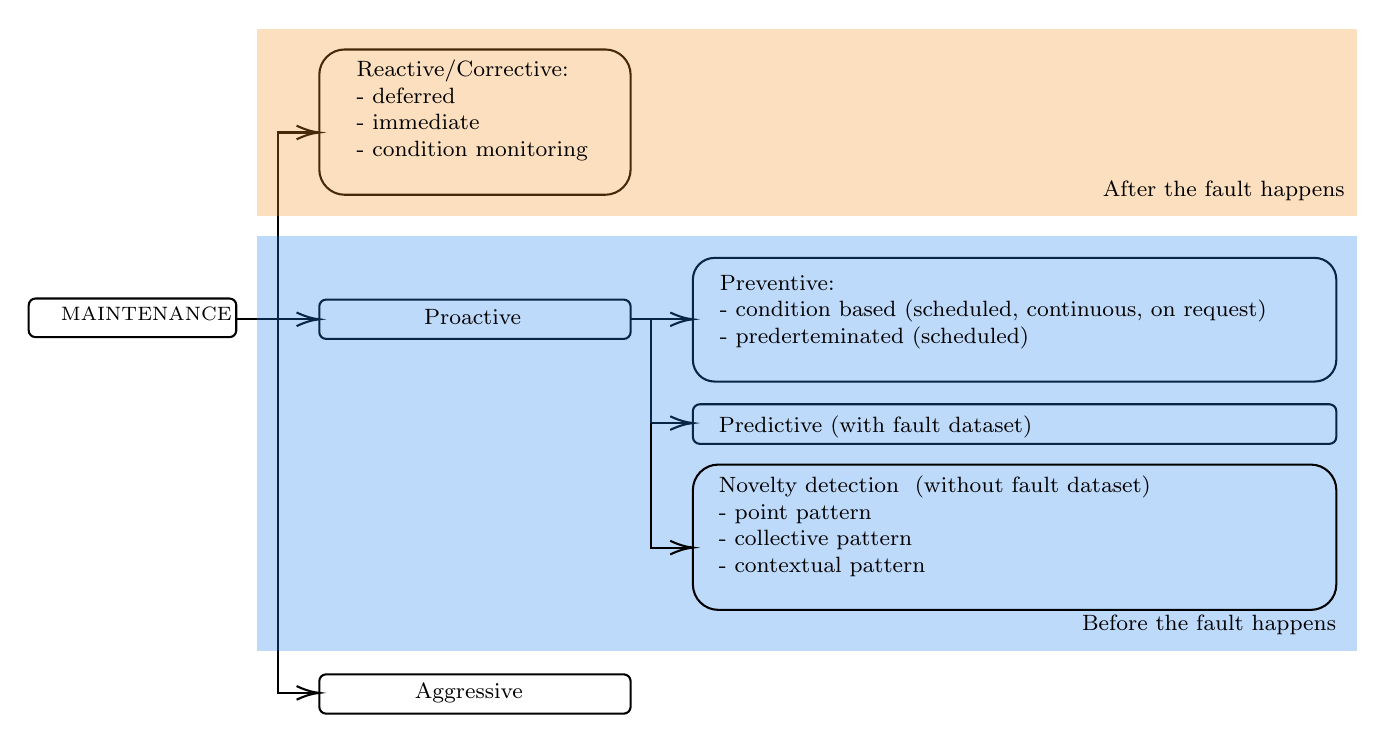
\begin{tikzpicture}[x=0.75pt,y=0.75pt,yscale=-1,xscale=1]
%uncomment if require: \path (0,472); %set diagram left start at 0, and has height of 472

%Flowchart: Alternative Process [id:dp19237775498206222] 
\draw   (110,143.25) .. controls (110,141.46) and (108.54,140) .. (106.75,140) -- (13.25,140) .. controls (11.46,140) and (10,141.46) .. (10,143.25) -- (10,155.34) .. controls (10,157.14) and (11.46,158.59) .. (13.25,158.59) -- (106.75,158.59) .. controls (108.54,158.59) and (110,157.14) .. (110,155.34) -- cycle ;
%Flowchart: Alternative Process [id:dp9736456094914503] 
\draw   (300,32.25) .. controls (300,25.48) and (294.52,20) .. (287.75,20) -- (162.25,20) .. controls (155.48,20) and (150,25.48) .. (150,32.25) -- (150,77.75) .. controls (150,84.52) and (155.48,90) .. (162.25,90) -- (287.75,90) .. controls (294.52,90) and (300,84.52) .. (300,77.75) -- cycle ;
%Flowchart: Alternative Process [id:dp14503627920432272] 
\draw   (300,143.83) .. controls (300,142) and (298.52,140.51) .. (296.68,140.51) -- (153.32,140.51) .. controls (151.48,140.51) and (150,142) .. (150,143.83) -- (150,156.14) .. controls (150,157.97) and (151.48,159.46) .. (153.32,159.46) -- (296.68,159.46) .. controls (298.52,159.46) and (300,157.97) .. (300,156.14) -- cycle ;
%Flowchart: Alternative Process [id:dp6071277747601995] 
\draw   (640,130.85) .. controls (640,125.09) and (635.33,120.42) .. (629.57,120.42) -- (340.43,120.42) .. controls (334.67,120.42) and (330,125.09) .. (330,130.85) -- (330,169.57) .. controls (330,175.33) and (334.67,180) .. (340.43,180) -- (629.57,180) .. controls (635.33,180) and (640,175.33) .. (640,169.57) -- cycle ;
%Flowchart: Alternative Process [id:dp2375215134913229] 
\draw   (640,194.29) .. controls (640,192.44) and (638.51,190.95) .. (636.67,190.95) -- (333.33,190.95) .. controls (331.49,190.95) and (330,192.44) .. (330,194.29) -- (330,206.67) .. controls (330,208.51) and (331.49,210) .. (333.33,210) -- (636.67,210) .. controls (638.51,210) and (640,208.51) .. (640,206.67) -- cycle ;
%Flowchart: Alternative Process [id:dp0632489558047773] 
\draw   (300,324.37) .. controls (300,322.54) and (298.52,321.06) .. (296.68,321.06) -- (153.32,321.06) .. controls (151.48,321.06) and (150,322.54) .. (150,324.37) -- (150,336.68) .. controls (150,338.52) and (151.48,340) .. (153.32,340) -- (296.68,340) .. controls (298.52,340) and (300,338.52) .. (300,336.68) -- cycle ;
%Straight Lines [id:da16540615986832674] 
\draw    (110,150) -- (130,150) -- (130,60) -- (148,60) ;
\draw [shift={(150,60)}, rotate = 180] [color={rgb, 255:red, 0; green, 0; blue, 0 }  ][line width=0.75]    (10.93,-3.29) .. controls (6.95,-1.4) and (3.31,-0.3) .. (0,0) .. controls (3.31,0.3) and (6.95,1.4) .. (10.93,3.29)   ;
%Straight Lines [id:da9369045726633412] 
\draw    (130,150) -- (148,150) ;
\draw [shift={(150,150)}, rotate = 180] [color={rgb, 255:red, 0; green, 0; blue, 0 }  ][line width=0.75]    (10.93,-3.29) .. controls (6.95,-1.4) and (3.31,-0.3) .. (0,0) .. controls (3.31,0.3) and (6.95,1.4) .. (10.93,3.29)   ;
%Straight Lines [id:da6629002710424032] 
\draw    (130,150) -- (130,330) -- (148,330) ;
\draw [shift={(150,330)}, rotate = 180] [color={rgb, 255:red, 0; green, 0; blue, 0 }  ][line width=0.75]    (10.93,-3.29) .. controls (6.95,-1.4) and (3.31,-0.3) .. (0,0) .. controls (3.31,0.3) and (6.95,1.4) .. (10.93,3.29)   ;
%Straight Lines [id:da30997716100450146] 
\draw    (300,150) -- (328,150) ;
\draw [shift={(330,150)}, rotate = 180] [color={rgb, 255:red, 0; green, 0; blue, 0 }  ][line width=0.75]    (10.93,-3.29) .. controls (6.95,-1.4) and (3.31,-0.3) .. (0,0) .. controls (3.31,0.3) and (6.95,1.4) .. (10.93,3.29)   ;
%Straight Lines [id:da8721835577612063] 
\draw    (310,150) -- (310,200) -- (328,200) ;
\draw [shift={(330,200)}, rotate = 180] [color={rgb, 255:red, 0; green, 0; blue, 0 }  ][line width=0.75]    (10.93,-3.29) .. controls (6.95,-1.4) and (3.31,-0.3) .. (0,0) .. controls (3.31,0.3) and (6.95,1.4) .. (10.93,3.29)   ;
%Shape: Rectangle [id:dp8985384381759749] 
\draw  [draw opacity=0][fill={rgb, 255:red, 241; green, 145; blue, 32 }  ,fill opacity=0.29 ] (120,10) -- (650,10) -- (650,100) -- (120,100) -- cycle ;
%Shape: Rectangle [id:dp08506626159443931] 
\draw  [draw opacity=0][fill={rgb, 255:red, 32; green, 129; blue, 241 }  ,fill opacity=0.29 ] (120,110) -- (650,110) -- (650,310) -- (120,310) -- cycle ;
%Flowchart: Alternative Process [id:dp46167581056222096] 
\draw   (640,232.25) .. controls (640,225.48) and (634.52,220) .. (627.75,220) -- (342.25,220) .. controls (335.48,220) and (330,225.48) .. (330,232.25) -- (330,277.75) .. controls (330,284.52) and (335.48,290) .. (342.25,290) -- (627.75,290) .. controls (634.52,290) and (640,284.52) .. (640,277.75) -- cycle ;
%Straight Lines [id:da5953849219282199] 
\draw    (310,200) -- (310,260) -- (328,260) ;
\draw [shift={(330,260)}, rotate = 180] [color={rgb, 255:red, 0; green, 0; blue, 0 }  ][line width=0.75]    (10.93,-3.29) .. controls (6.95,-1.4) and (3.31,-0.3) .. (0,0) .. controls (3.31,0.3) and (6.95,1.4) .. (10.93,3.29)   ;

% Text Node
\draw (341.5,127.21) node [anchor=north west][inner sep=0.75pt]  [font=\fontsize{0.8em}{0.96em}\selectfont] [align=left] {Preventive:\\\mbox{-} condition based (scheduled, continuous, on request)\\\mbox{-} prederteminated (scheduled)};
% Text Node
\draw (24,142.8) node [anchor=north west][inner sep=0.75pt]  [font=\fontsize{0.8em}{0.96em}\selectfont] [align=left] {{\fontsize{0.8em}{0.96em}\selectfont MAINTENANCE}};
% Text Node
\draw (199,143.49) node [anchor=north west][inner sep=0.75pt]  [font=\fontsize{0.8em}{0.96em}\selectfont] [align=left] {Proactive};
% Text Node
\draw (194.5,324.03) node [anchor=north west][inner sep=0.75pt]  [font=\fontsize{0.8em}{0.96em}\selectfont] [align=left] {Aggressive};
% Text Node
\draw (341,195) node [anchor=north west][inner sep=0.75pt]  [font=\fontsize{0.8em}{0.96em}\selectfont] [align=left] {Predictive (with fault dataset)};
% Text Node
\draw (166.5,23.5) node [anchor=north west][inner sep=0.75pt]  [font=\fontsize{0.8em}{0.96em}\selectfont] [align=left] {Reactive/Corrective:\\\mbox{-} deferred\\\mbox{-} immediate\\\mbox{-} condition monitoring};
% Text Node
\draw (516,291) node [anchor=north west][inner sep=0.75pt]   [align=left] {{\fontsize{0.8em}{0.96em}\selectfont Before the fault happens}};
% Text Node
\draw (526,82) node [anchor=north west][inner sep=0.75pt]   [align=left] {{\fontsize{0.8em}{0.96em}\selectfont After the fault happens}};
% Text Node
\draw (341,224.05) node [anchor=north west][inner sep=0.75pt]  [font=\fontsize{0.8em}{0.96em}\selectfont] [align=left] {Novelty detection \ (without fault dataset)\\\mbox{-} point pattern\\\mbox{-} collective pattern\\\mbox{-} contextual pattern};


\end{tikzpicture}
    \caption{Maintenance techniques}
    \label{fig:maintthechniques}
\end{figure}